%\documentclass[oneside, final, 12pt]{extreport}
\documentclass[12pt,fleqn]{article}

\usepackage{amsmath, amsthm, amssymb} %math expressions, theoreme/lemma, math symbols
\usepackage{mathtext} %russian letters in formulas

% fonts and lang
%\usepackage[T1,TS1,T2A]{fontenc}
\usepackage{cmap}
\usepackage[T1, T2A]{fontenc}
\usepackage[utf8]{inputenc}
\usepackage[english, russian]{babel}


% formatting
% \usepackage{geometry} %customize page layout
% \geometry{left = 3cm}
% \geometry{right = 1cm}
% \geometry{top = 1.5cm}
% \geometry{bottom = 2cm}

\usepackage{setspace} %set space between lines
\usepackage{indentfirst} %indent first pagearagraph after section header

\usepackage{tocloft} %control table of contents, figures

\usepackage{graphicx}

\usepackage{hhline}

\usepackage{caption}

\usepackage{subcaption}

\usepackage[shortlabels]{enumitem}
\setlist{nolistsep, itemsep=0.1cm, parsep=0pt, leftmargin=1.5cm}

\usepackage{multirow}

\usepackage{algorithm}
\usepackage{algpseudocode}

\textheight=25cm
\textwidth=16cm
\oddsidemargin=5mm % левое поле для нечётных страниц
\evensidemargin=-5mm % севое поле для чётных страниц
%\marginparwidth=36pt
\topmargin=-3cm % расстояние от верхней границы листа до заголовка
%\flushbottom % выстота тела всех страниц одинаковая 
\raggedbottom % позволяет несколько различаться высоте тел различных страниц
\tolerance 3000 % how much badness is allowable without error. 

\linespread{1.3} %1.5 spacing 

\parindent 1.27cm % Абзацный отступ

\sloppy             % текст редко залезает на правое поле
\clubpenalty = 10000  % Запрещаем разрыв страницы после первой строки абзаца
\widowpenalty = 10000 % Запрещаем разрыв страницы после предпоследней строки абзаца
% \global\hyphenpenalty = 1000 % Частота переносов

\usepackage{listings}
\lstset{
    %numbers=left,
    breaklines=true,
    %backgroundcolor=\color{light-gray},
    tabsize=3
}


%Разработка метода прогнозирования слабой масштабируемости суперкомпьютерных приложений

\begin{document}

	\begin{titlepage}
	\begin{center}
		
\includegraphics[width=50mm]{./images/MSU}

	    Московский государственный университет имени М.В.Ломоносова

	    %\bigskip
	    Факультет вычислительной математики и кибернетики

	    Кафедра суперкомпьютеров и квантовой информатики\\[20mm]

	    %{\largeМокров Кирилл Сергеевич}\\[5mm]

	    %\textsf{\Large\bfseriesКурс - Параллельные высокопроизводительные вычисления}\\[15mm]
	    {Практическое задание 1.\\Параллельная реализация операций с сеточными данными\\на неструктурированной смешанной сетке }\\[35mm]

	    \begin{flushright}
	        %\parbox{0.5\textwidth}{
	            % Выполнил:\\
	            % студент 4 курса 423 группы\\
	            % \emph{Мокров Кирилл Сергеевич}\\[5mm]
	            
	            Мокров Кирилл Сергеевич\\
	            523 группа\\
	            Дата подачи: ???
	            
	        %}
	    \end{flushright}
	       

	    \vspace{\fill}
	    Москва, 2020
	\end{center}
\end{titlepage}

\clearpage
%\newpage

	\tableofcontents
	\thispagestyle{empty}
	\clearpage
	\setcounter{page}{3}

	\section{Описание задания и программной реализации}
	\subsection{Краткое описание задания}
		Задание можно разбить на 4 этапа:
		\begin{enumerate}
			\item Generate - генерация графа/портрета по тестовой сетке. По двумерной неструктурированной смешанной сетке, состоящей из треугольников и четырёхугольников генерируется портрет разреженной матрицы смежности графа, дополненный главной диагональю в формате CSR.
			\item Fill - заполнение матрицы и вектора правой части по заданному портрету.
			\item Solve - решение СЛАУ с полученной матрицей. Так как матрица, полученная на предыдущем этапе, симметричная, то используется метод сопряженных градиентов с предобуславливателем Якоби.
			\item Report - проверка корректности и выдача измерений. Проверка, что невязка системы после работы решателя удовлетворяет заданной точности, выдача значения невязки и печать таблицы таймирования всех предыдущих этапов.

		\end{enumerate}

	\subsection{Краткое описание программной реализации}
		Сначала в функции \textit{main} происходит считывание данных командной строки, проверка их корректности и выдача диагностики. Параметры программы: \textit{Nx}, \textit{Ny}, \textit{K1}, \textit{K2}. Их значение хорошо поясняет рисунок \ref{param}. В случае параллельной реализации после них ещё идёт количество используемых нитей. А в самом конце может быть необязательный аргумент включающий отладочную печать.
			\begin{figure}[H]
		        \centering
		        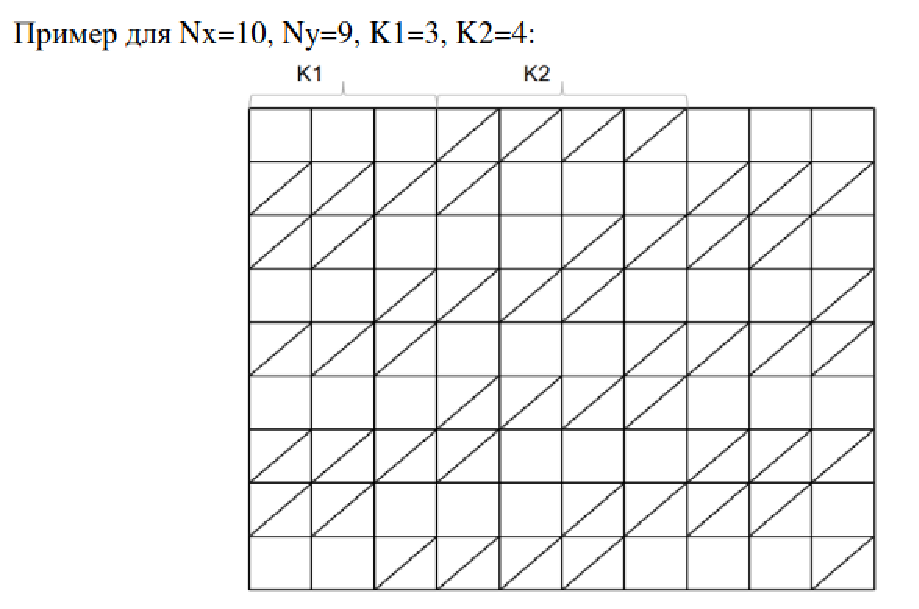
\includegraphics[width=0.5\textwidth]{./images/param}
		        \caption{Параметры командной строки}
		        \label{param}
		    \end{figure}

	\begin{lstlisting}[numbersep=10pt, language=C++, caption=\textbf{Реализованные функции}]
// Inner product of two vectors vec_1 ans vec_2
double dotKernel(const std::vector<double>& vec_1, const std::vector<double>& vec_2);

// Linear combination of two vectors x = a * x + b * y
void axpbyKernel(const double a, std::vector<double>& x,
	             const double b, const std::vector<double>& y);

// Matrix vector product with sparse matrix. row_ptr, col_ptr - CSR representation, res = Matrix * vec
void SpMVKernel(const std::vector<double>& matrix, const std::vector<int>& row_ptr, const std::vector<int>& col_ptr, const std::vector<double>& vec, std::vector<double>& res);

// Compution, how many cells with obliques line before cell with index cell_idx, K1, K2 - parameters that determine the distribution of oblique lines
int obliquesBefore(const int K1, const int K2, const int cell_idx);

// Determines whether a cell with the cell_idx index contains oblique line,  K1, K2 - parameters that determine the distribution of oblique lines
bool hasOblique(const int K1, const int K2, const int cell_idx);

// Function corresponds to the first stage of the task. Nx, Ny, K1, K2 - determine the configuration of a two-dimensional grid, row_ptr, col_ptr - CSR representation
void generate(const int Nx, const int Ny, const int K1, const int K2, std::vector<int>& row_ptr, std::vector<int>& col_ptr);

// Function corresponds to the second stage of the task. Nx, Ny - determine grid size, row_ptr, col_ptr - CSR representation, A_arr, b_vec - fillable matrix and vector
void fill(const int Nx, const int Ny, const std::vector<int>& row_ptr, const std::vector<int>& col_ptr, std::vector<double>& A_arr, std::vector<double>& b_vec);

// Function corresponds to the third stage of the task. A_arr, b_vec - initial data for solving systems of linear equations, row_ptr, col_ptr - CSR representation, x_vec - equations solution, TOL - relative error of the solution
void Solve(const std::vector<double>& A_arr, const std::vector<double>& b_vec, const std::vector<int>& row_ptr, const std::vector<int>& col_ptr, std::vector<double>& x_vec, const double TOL = 1e-4);
	\end{lstlisting}
\section{Исследование производительности}
	\subsection{Характеристики вычислительной системы}
	Тестирования программы проводились на вычислительном комплексе \textit{IBM Polus}. Polus - параллельная вычислительная система, состоящая из 5 вычислительных узлов. Каждый узел оборудован двумя десятиядерными процессорами \textit{IBM Power 8}, каждое ядро которого имеет 8 потоков, 256 GB оперативной памяти. Производительность кластера (TFlop/s): 55,84 (пиковая), 40,39 (Linpack).
	\subsection{Результаты измерений производительности}
		\subsubsection{Последовательная производительность}
		\begin{table}[H]
			\begin{tabular}{|c||c|c|c|c|c|c|}
				\hline
				\multirow{2}{*}{N} &  \multirow{2}{*}{Generation} & \multirow{2}{*}{Filling} & Dot & Axpby & SpMV          & \multirow{2}{*}{Memory} \\ \cline{4-6}
				                   &                              &                         & \multicolumn{3}{c|}{Solver}  &                         \\ \hline
                \multirow{2}{*}{10000} & \multirow{2}{*}{0.000106} & \multirow{2}{*}{0.002573} & 0.000472 & 0.000278 & 0.001478              & \multirow{2}{*}{1.37} \\ \cline{4-6}
                                       &                     &                    & \multicolumn{3}{c|}{0.002410} &               \\ \hline
                \multirow{2}{*}{100000} &  \multirow{2}{*}{0.000942} & \multirow{2}{*}{0.029858} & 0.004723 & 0.002842 & 0.014849 & \multirow{2}{*}{12.65} \\ \cline{4-6}
                                      &                     &                     & \multicolumn{3}{c|}{0.023946} &  \\ \hline
                \multirow{2}{*}{1000000} &  \multirow{2}{*}{0.009342} & \multirow{2}{*}{0.302991} & 0.051984 & 0.032798 & 0.163295 & \multirow{2}{*}{124.66} \\ \cline{4-6}
                                       &                     &                    & \multicolumn{3}{c|}{0.263362} &  \\ \hline
                \multirow{2}{*}{10000000} &  \multirow{2}{*}{0.086874} & \multirow{2}{*}{3.014130} & 0.517145 & 0.326723 & 1.640600 & \multirow{2}{*}{1224.79} \\ \cline{4-6}
                                       &                     &                    & \multicolumn{3}{c|}{2.622970} &  \\ \hline
			\end{tabular}
			\caption{Время (в секундах) работы 3 этапов программы, 3 основных вычислительных ядер и затраченная на работу всей программы память (в MB)}
			\label{seq}
		\end{table}
		По результатам, представленным в таблице \ref{seq}, видно, что с ростом размера задачи время этапов инициализации, основных ядер солвера, количества использованной памяти растёт линейно.
        \begin{figure}[H]
            \centering
            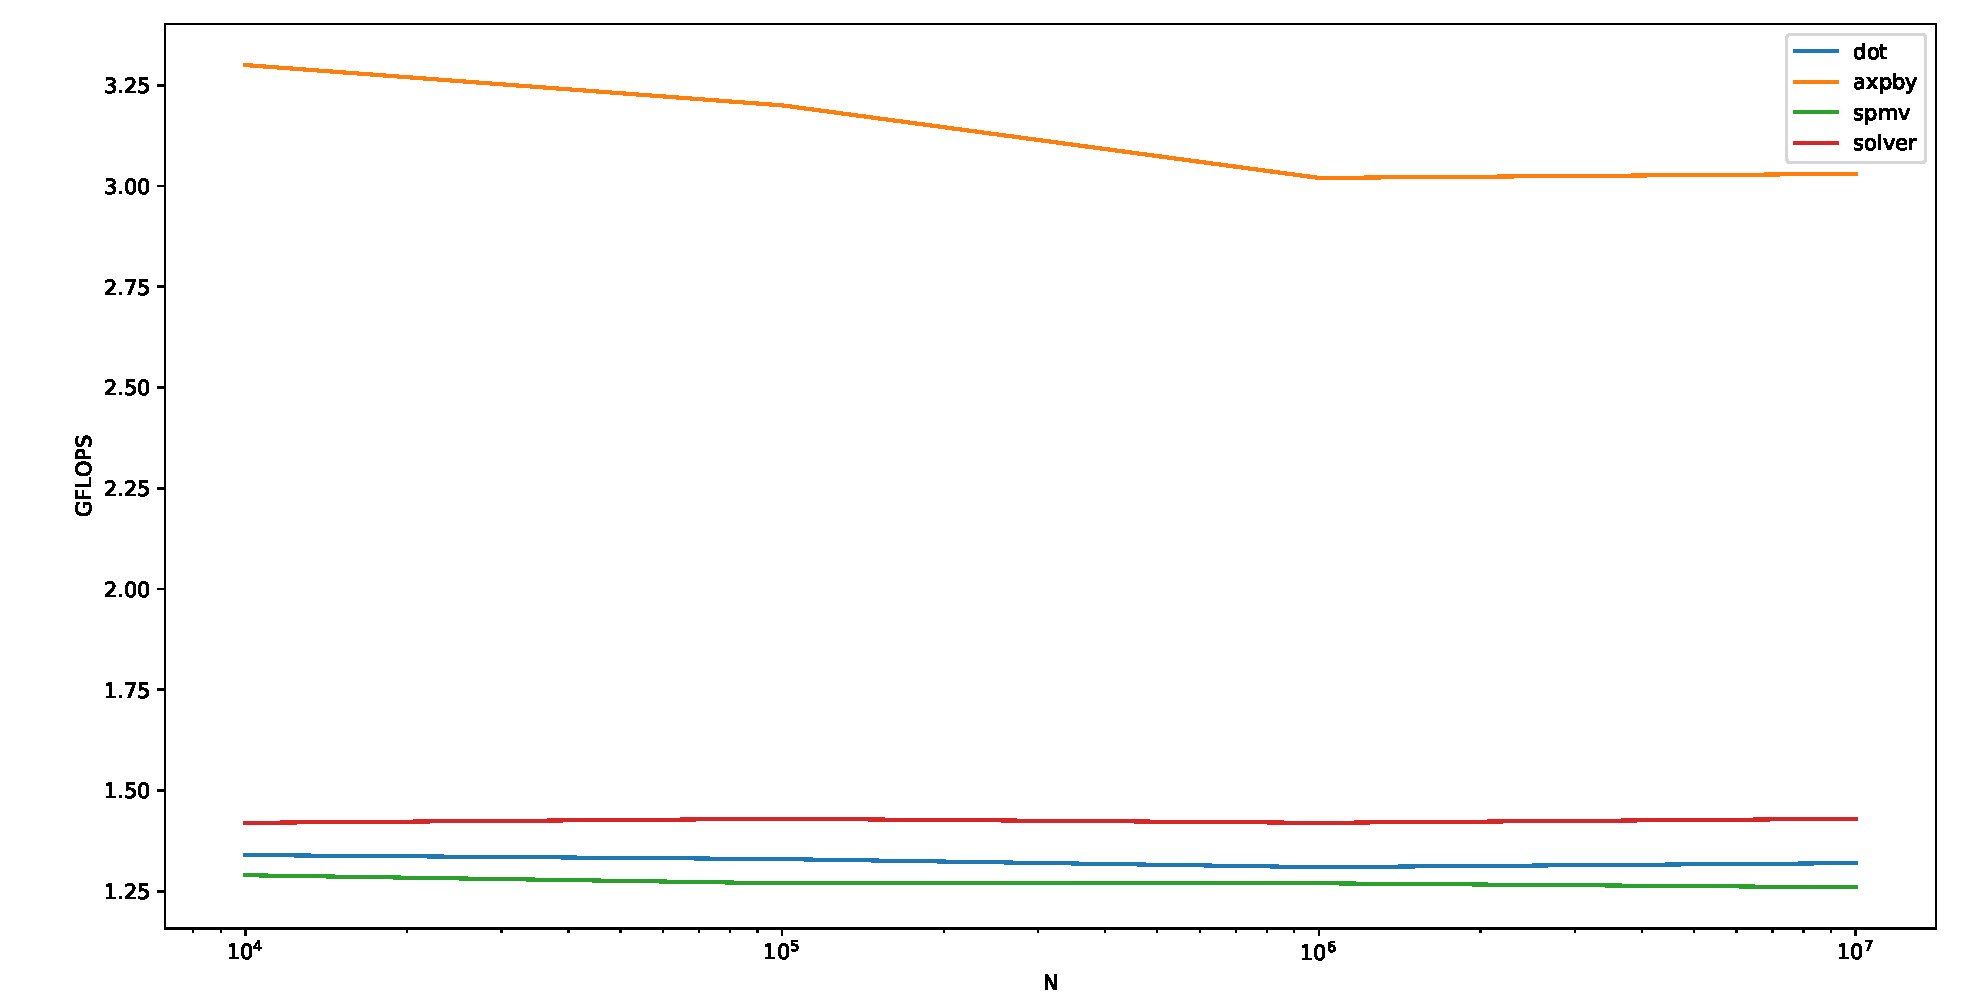
\includegraphics[width=0.9\textwidth]{./images/seq_perf}
            \caption{Производительность 3 основных вычислительных ядер и всего солвера}
            % \label{figure_HPL_C_3}
        \end{figure}
		\subsubsection{Параллельное ускорение}
		\begin{table}[H]
			\centering
			\begin{tabular}{|c||c|c|c|c|c|}
				\hline
				\multirow{2}{*}{T} &  \multirow{2}{*}{Generation | S-up} & \multirow{2}{*}{Filling | S-up} & Dot | S-up & Axpby | S-up & SpMV | S-up \\ \cline{4-6}
				                   &                              &                         & \multicolumn{3}{c|}{Solver | S-up} \\ \hline
                \multirow{2}{*}{1} & \multirow{2}{*}{1544 | 1,0} & \multirow{2}{*}{30508 | 1,0} & 4753 | 1,0 & 2085 | 1,0 & 14625 | 1,0 \\ \cline{4-6}
                                   &                   &                   & \multicolumn{3}{c|}{22796 | 1,0}   \\ \hline
                \multirow{2}{*}{2} & \multirow{2}{*}{847 | 1,8} & \multirow{2}{*}{15308 | 2,0} & 2397 | 1,9 & 2128 | 0,97 & 7356 |  1,9\\ \cline{4-6}
                                   &                   &                   & \multicolumn{3}{c|}{12836| 1,7}   \\ \hline
                \multirow{2}{*}{4} & \multirow{2}{*}{471 | 3,3} & \multirow{2}{*}{7697 | 3,9} & 1262 | 3,7& 1144 | 1,8& 3768 | 3,9\\ \cline{4-6}
                                   &                   &                   & \multicolumn{3}{c|}{7005| 3,2}   \\ \hline
                \multirow{2}{*}{8} & \multirow{2}{*}{436 | 3,6} & \multirow{2}{*}{3886 | 7,8} & 774 | 6,1& 726 | 2,9& 2067 |  7,0\\ \cline{4-6}
                                   &                   &                   & \multicolumn{3}{c|}{4350| 5,2}   \\ \hline
                \multirow{2}{*}{16} & \multirow{2}{*}{518 | 3,0} & \multirow{2}{*}{2252 | 13,5} & 674 | 7,0& 707 | 2,9& 1572 |  9,3\\ \cline{4-6}
                                   &                   &                   & \multicolumn{3}{c|}{3858| 5,9}   \\ \hline
                \multirow{2}{*}{32} & \multirow{2}{*}{799 | 1,9} & \multirow{2}{*}{1551 | 19,6} & 819 | 5,8& 774 | 2,7& 1472 |  9,9\\ \cline{4-6}
                                   &                   &                   & \multicolumn{3}{c|}{3962| 5,7}   \\ \hline

			\end{tabular}
			\caption{Время (в мкс) работы и ускорение 3 этапов программы и 3 основных вычислительных ядер, N = 100'000}
			\label{par_1}
		\end{table}
		\begin{table}[H]
			\begin{tabular}{|c||c|c|c|c|c|}
				\hline
				\multirow{2}{*}{T} &  \multirow{2}{*}{Generation | S-up} & \multirow{2}{*}{Filling | S-up} & Dot | S-up & Axpby | S-up & SpMV | S-up \\ \cline{4-6}
				                   &                              &                         & \multicolumn{3}{c|}{Solver | S-up} \\ \hline
                \multirow{2}{*}{1} & \multirow{2}{*}{1581610 | 1,0} & \multirow{2}{*}{3104950 | 1,0} & 473064 | 1,0 & 212899 | 1,0 & 1434150 | 1,0 \\ \cline{4-6}
                                   &                   &                   & \multicolumn{3}{c|}{2259050 | 1,0}   \\ \hline
                \multirow{2}{*}{2} & \multirow{2}{*}{791180 | 2,0} & \multirow{2}{*}{1566810| 1,9} & 239733 | 1,9 & 211287 | 1,0& 716838 | 2,0 \\ \cline{4-6}
                                   &                   &                   & \multicolumn{3}{c|}{1259280 | 1,8}   \\ \hline
                \multirow{2}{*}{4} & \multirow{2}{*}{397837 | 3,9} & \multirow{2}{*}{782295 | 3,9} & 123937 | 3,8& 114709 | 1,8& 402956 | 3,5 \\ \cline{4-6}
                                   &                   &                   & \multicolumn{3}{c|}{706907 | 3,2}   \\ \hline
                \multirow{2}{*}{8} & \multirow{2}{*}{209928 | 7,5} & \multirow{2}{*}{401158 | 7,7} & 63847 | 7,4& 70197 | 3,0& 188113 |  7,6\\ \cline{4-6}
                                   &                   &                   & \multicolumn{3}{c|}{378095 | 6,0}   \\ \hline
                \multirow{2}{*}{16} & \multirow{2}{*}{159830 | 9,9} & \multirow{2}{*}{238812 | 13,0} & 56495 | 8,3& 67089 | 3,1& 160765 |  8,9\\ \cline{4-6}
                                   &                   &                   & \multicolumn{3}{c|}{340134 | 6,6}   \\ \hline
                \multirow{2}{*}{32} & \multirow{2}{*}{168950 | 9,3} & \multirow{2}{*}{167382 | 18,5} & 54456 | 8,6& 65948 | 3,2& 170258 |  8,4\\ \cline{4-6}
                                   &                   &                   & \multicolumn{3}{c|}{349474 | 6,4}   \\ \hline

			\end{tabular}
			\caption{Время (в мкс) работы и ускорение 3 этапов программы и 3 основных вычислительных ядер, N = 10'000'000}
			\label{par_2}
		\end{table}
		В таблицах \ref{par_1} и \ref{par_2} представлены время работы параллельной программы на \(1, 2, 4, 8, 16, 32\) нитях, при \(N = 10^5\) и \(N = 10^7\). Не самое хорошее ускорение некоторых этапов работы программы в первом случае можно объяснить небольшим размером задачи, иногда бывает выгодней использовать меньше нитей, но в то же время тратить меньше времени на манипуляции с ними. Для второго же случая, задача ощутимо лучше распараллеливается, ускорение для некоторых этапов доходит до 9 - 18 раз.
		\begin{table}[H]
			\begin{tabular}{|c||c|c|c|c|c|c|}
				\hline
				& \multicolumn{6}{|c|}{Nx, Ny, K1, K2} \\ \hline
				   & \multicolumn{3}{c|}{100, 1000, 15, 4} & \multicolumn{3}{c|}{1000, 10000, 15, 4} \\ \hline
				T  & DOT   & AXPBY &  SpMV &   DOT & AXPBY & SpMV \\ \hline
				1  & 1,302 & 4,205 & 1,48  & 1,312 & 4,090 & 1,512 \\ \hline
				2  & 2,604 & 4,118 & 2,96  & 2,589 & 4,112 & 3,026 \\ \hline
				4  & 4,960 & 7,685 & 5,78  & 5,008 & 7,592 & 5,384 \\ \hline
				8  & 8,091 & 12,09 & 10,5  & 9,721 & 12,40 & 11,53 \\ \hline
				16 & 9,300 & 12,44 & 13,8  & 10,98 & 12,98 & 13,49 \\ \hline
				32 & 7,626 & 11,34 & \textit{14,8}  & \textit{11,39} & \textit{13,20} & 12,74 \\ \hline
			\end{tabular}
			\caption{Производительность трёх основных вычислительных ядер, GFlops\\(лучшие результаты выделены курсивом)}
			\label{real_perf}
		\end{table}
\section{Анализ полученных результатов}
	Для начала рассчитаем \(TBP = min(TPP, BW \dot AI)\). На \textit{Polus} используется процессор \textit{Power 8}, обнаружить в интернете, какими векторными расширениями обладает данный процессор не удалось, поэтому предположим, что одной его ядро располагает двумя \textit{AVX512}. Тогда так как это 10 ядерный процессор, частоты работы которого могут изменяться от 2.5GHz  до 5GHz, \(TPP\) можно посчитать так: \(TPP = 10C * 2.5GHz * 2 * 512 / 64 = 400 GFlops\). За \(BW\) возьмём пропускную способность контроллера памяти - 230 GB/s.

	Расчёт AI. Пусть X - длина вектора \(row\_ptr\), Y - \(col\_ptr\). DOT: цикл размера X, с телом sum = sum + a[i] * b[i], FLOP - 2 * X (сложение и умножение), BYTE - 2 * X * 8 (два вектора a, b). AXPBY: цикл размера Х, с телом x[i] = a * x[i] + b * y[i], FLOP - 3 * X (два умножения и сложение), BYTE - 3 * X * 8 (два вектора прочитать, один записать). SpMV: вложенные циклы, если представить их одним, то его размер будет Y, тело sum = sum + a[i] * b[i], FLOP - 2 * Y (сложение и умножение), BYTE - 8 * (Y + 2X) + 4 * (Y + X) (матрица, \(col\_ptr\) по Y, \(row\_ptr\), vec, res по Х).
	\begin{table}[H]
		\centering
		\begin{tabular}{|c||c|c|c|c|c|c|}
			\hline
			Kernel & AI, Flop / byte & TBP, GFlops & \%,TBP & \%, TPP \\ \hline
			dot    &           0.125 &       28.75 & 40 & 2,8 \\ \hline
			axpby  &           0.130 &       29.90 & 44 & 3,3 \\ \hline
			spmv   &           0.098 &       22.54 & 65 & 3,7 \\ \hline
		\end{tabular}
		\caption{AI, TBP и количество процентов от достижимой и пиковой производительностей для трёх основных вычислительных ядер}
	\end{table}
	Для вычислительных ядер проценты от достижимой производительности достаточно велики, от 40 до 65. Если же рассматривать пиковую производительность, то всё сильно хуже, и это несмотря на то, что при расчётах использовались минимальная тактовая частота и максимальная пропускная способность процессора.

\clearpage
%\newpage

\end{document}